\documentclass[12pt]{exam}
\usepackage[utf8]{inputenc}
\usepackage{amsmath,amstext,amsthm,amssymb,amsxtra, graphicx}
\usepackage[top=1.5in, bottom=1.5in, left=1.25in, right=1.25in]	{geometry}
%\usepackage[normalem]{ulem}
\usepackage{txfonts} % pxfonts txfonts 
\usepackage[T1]{fontenc}
\usepackage{lmodern}
\renewcommand*\familydefault{\sfdefault}
 \usepackage{euler}   % better than the option below
\usepackage{pdfsync}
\usepackage{multicol}
\newcommand{\ci}[1]{_{ {}_{\scriptstyle #1}}}
\graphicspath{ {images/} }


\newcommand{\norm}[1]{\ensuremath{\left\|#1\right\|}}
\newcommand{\abs}[1]{\ensuremath{\left\vert#1\right\vert}}
\newcommand{\ip}[2]{\ensuremath{\left\langle#1,#2\right\rangle}}
\newcommand{\p}{\ensuremath{\partial}}
\newcommand{\pr}{\mathcal{P}}

\newcommand{\pbar}{\ensuremath{\bar{\partial}}}
\newcommand{\db}{\overline\partial}
\newcommand{\D}{\mathbb{D}}
\newcommand{\B}{\mathbb{B}}
\newcommand{\Sp}{\mathbb{S}}
\newcommand{\T}{\mathbb{T}}
\newcommand{\R}{\mathbb{R}}
\newcommand{\Z}{\mathbb{Z}}
\newcommand{\C}{\mathbb{C}}
\newcommand{\N}{\mathbb{N}}
\newcommand{\Q}{\mathbb{Q}}
\newcommand{\mQ}{\mathcal{Q}}
\newcommand{\mS}{\mathcal{S}}
\newcommand{\scrH}{\mathcal{H}}
\newcommand{\scrL}{\mathcal{L}}
\newcommand{\td}{\widetilde\Delta}
\newcommand{\pw}{\text{PW}}
\newcommand{\esup}{\text{ess.sup}}
\newcommand{\Tn}{\mathcal{T}_n}
\newcommand{\Bn}{\mathbb{B}_n}
\newcommand{\rt}{\mathcal{O}}
\newcommand{\avg}[1]{\langle #1 \rangle}
\newcommand{\one}{\mathbbm{1}}
\newcommand{\eps}{\varepsilon}
\newcommand{\grad}{\nabla}

\newcommand{\La}{\langle }
\newcommand{\Ra}{\rangle }
\newcommand{\rk}{\operatorname{rk}}
\newcommand{\card}{\operatorname{card}}
\newcommand{\ran}{\operatorname{Ran}}
\newcommand{\osc}{\operatorname{OSC}}
\newcommand{\im}{\operatorname{Im}}
\newcommand{\re}{\operatorname{Re}}
\newcommand{\tr}{\operatorname{tr}}
\newcommand{\vf}{\varphi}
\newcommand{\f}[2]{\ensuremath{\frac{#1}{#2}}}

\newcommand{\kzp}{k_z^{(p,\alpha)}}
\newcommand{\klp}{k_{\lambda_i}^{(p,\alpha)}}
\newcommand{\TTp}{\mathcal{T}_p}
\newcommand{\m}[1]{\mathcal{#1}}
\newcommand{\md}{\mathcal{D}}
\newcommand{\qan}{\abs{Q}^{\alpha/n}}
\newcommand{\sbump}[2]{[[ #1,#2 ]]}
\newcommand{\mbump}[2]{\lceil #1,#2 \rceil}
\newcommand{\cbump}[2]{\lfloor #1,#2 \rfloor}

\newcommand{\hn}{{4}}
\newcommand{\dd}{{10-28}}
\newcommand{\class}{Aero 417}
\newcommand{\term}{Fall 2024}
\newcommand{\examnum}{Homework \hn: Due \dd}
\newcommand{\examdate}{}
\newcommand{\timelimit}{75 Minutes}
\newcommand{\vc}[3]{\langle #1,#2,#3\rangle}
\newcommand*{\vv}[1]{\vec{\mkern0mu#1}}
\newcommand{\bv}[1]{\boldsymbol{#1}}
\newcommand{\hide}[1]{}
\newcommand{\uvec}[1]{\boldsymbol{\hat{\textbf{#1}}}}
\newcommand{\vex}[1]{\boldsymbol{{\textbf{#1}}}}
\newcommand{\px}{\frac{\partial}{\partial x}}
\newcommand{\py}{\frac{\partial}{\partial y}}
\newcommand{\pt}{\frac{\partial}{\partial t}}
\newcommand{\pxx}{\frac{\partial^2}{\partial x^2}}
\newcommand{\pyy}{\frac{\partial^2}{\partial y^2}}
\newcommand{\ptt}{\frac{\partial^2}{\partial t^2}}


\pagestyle{head}
\firstpageheader{}{}{}
\runningheader{\class}{ Page \thepage\ of \numpages}{\examnum}
\runningheadrule

\makeatletter
\renewcommand*\env@matrix[1][*\c@MaxMatrixCols c]{%
  \hskip -\arraycolsep
  \let\@ifnextchar\new@ifnextchar
  \array{#1}}
\makeatother

\printanswers
\begin{document}

\noindent
\begin{tabular*}{\textwidth}{l @{\extracolsep{\fill}} r @{\extracolsep{6pt}} l}
\textbf{\class} & \textbf{Name:} & \makebox[2in]{\bf{Benjamin Tollison}}\\
\end{tabular*}\\
\rule[2ex]{\textwidth}{2pt}
%
\begin{questions}
\begin{question}
Comparing centrifugal and axial compressors, what is the reason in which centrifugal
compressor presents higher pressure ratio per stage than axial compressors?
\end{question}
\begin{solutionorbox}[\stretch{1}]
The main diffence in a single stage of an axial compressor vs a centrifugal compressor
is the how the airflow travels through the stage. With axial compressors, the flow runs parrellel to
throughout the stage, whereas in a centrifugal compressor the flow is turned. This extra turning
allows for more kinectic energy to be increased more in the same amount of space. This radial 
acceleration of the flow imparts more total pressure and total velocity on the working gas 
in a single stage compared to an axial stage.
\end{solutionorbox}

\newpage 
\begin{question}
Based on a specific axial compressor design requirement, describe with details the procedure
to obtain an adequate preliminary 3D turbomachine sizing. Also, create a diagram of this
project process.
\end{question}
\begin{solutionorbox}[\stretch{1}]
\[
\text{Design Point} = f\left(\phi,\psi,\bar{w},M_{tip}\right)
\]
Where the ratio between the axial flow and the actual velocity across the blade is defined as: 
\[\phi = \frac{V_{axial}}{U}\]
Work coefficient is the ratio of specific work over kinectic energy:
\[\psi = \frac{-\Delta{h_0}}{\frac{U^2}{2}} \Rightarrow 2\phi \left(\tan{\alpha_1} - \tan{\alpha_2}\right)\]
Load coefficient is \(\bar{w} = \frac{\psi}{2}\) and Mach number at the rotor tip is \(M_{tip} = \frac{U_{tip}}{\sqrt{\gamma RT}}\)
These parameters are what we can desing the compressor around in order to get the desired \(\Delta{h_0}\) that we want.
\\
The process to determind the intial design is to first identifying the altitude and speed that the aircraft should be flying at for cruise.
Then that will give us \(\rho,T_0,P_0,V_{axial}\). From there we can choose a design \(\pi_{0,C}\) and that will tell us the required \(\Delta{h_0}\) with:
\[\pi_{0,C} = \frac{T_2}{T_1}^\frac{\gamma}{\gamma-1} \approx \frac{h_2}{h_1}^\frac{\gamma}{\gamma-1}\]
\[\therefore h_2 - h_1 = h_1 \pi_{0,C}^\frac{\gamma-1}{\gamma} - h_1\]
From there we can adjust the rpm, rotor, and stators angles until we get the design work coefficient. With
the rpm, and the turning angles we can then make our 3-D design and do a CFD analysis to refine the desired pressure ratio.
After the simulation model is finallized, then we can move on to wind tunnel testing. The wind tunnel testing will either verify our design, or
make us change the rpm, and turning angles. This process repeats until we get something that can be pushed to production.
\\
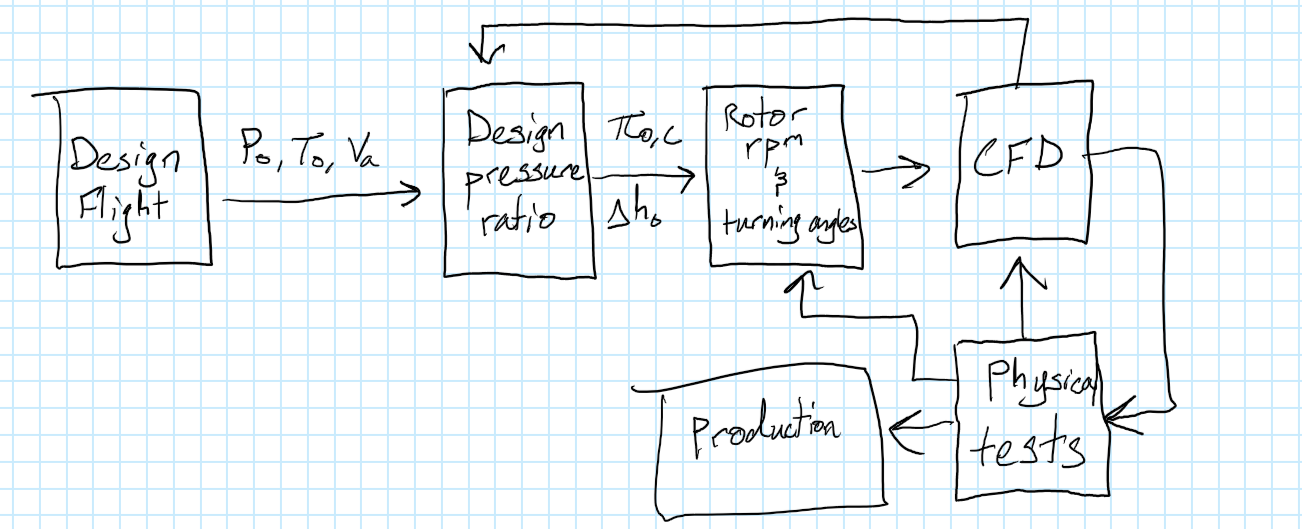
\includegraphics[width = \linewidth]{hand drawn production cycle.png}
\end{solutionorbox}


\newpage 
\begin{question}
What is the objective in the use of variable geometry (VIGV and VSV)?
\end{question}
\begin{solutionorbox}[\stretch{1}]
Due to a go amount of time that an engine will not operating at it's design point, we need to 
maximize the efficiency of the engine during these times.
\[
\pi_{0C}, \eta_C = f \left( \frac{\dot{m} \sqrt{T_{01}}}{p_{01}}, M_{tip} \right).
\]
The efficiency of the compressor is going to be dictated by avoiding un-wanted shock waves and flow
separation we can increase the angles of the stators to impart more work on the gas at lower speeds than 
the design point and decrease the angles on the stators at higher speeds than the design point in order to 
prevent flow separation. Decreasing the angles of the stators at higher speeds also prevent strong shock waves 
from forming that dramatically decrease the total pressure coming out, which therefore would decrease the overall efficiency.
\end{solutionorbox}


\newpage 
\begin{question}
In a compressor operational map, for each rotational speed there are two limit points, stall
and choke. Make a sketch of a compressor map with different rotational speeds, identifying
these points including the stall/surge line and explain the physical aspects of stall, surge and
choke.
\end{question}
\begin{solutionorbox}[\stretch{1}]
The surge line is how far you can pull the angle of attack and the turning angles to maximize the pressure ratio of the compressor
before flow separation overwelms the compressor and not enough mass flow is making it to the turbine to keep the cycle running.
\\
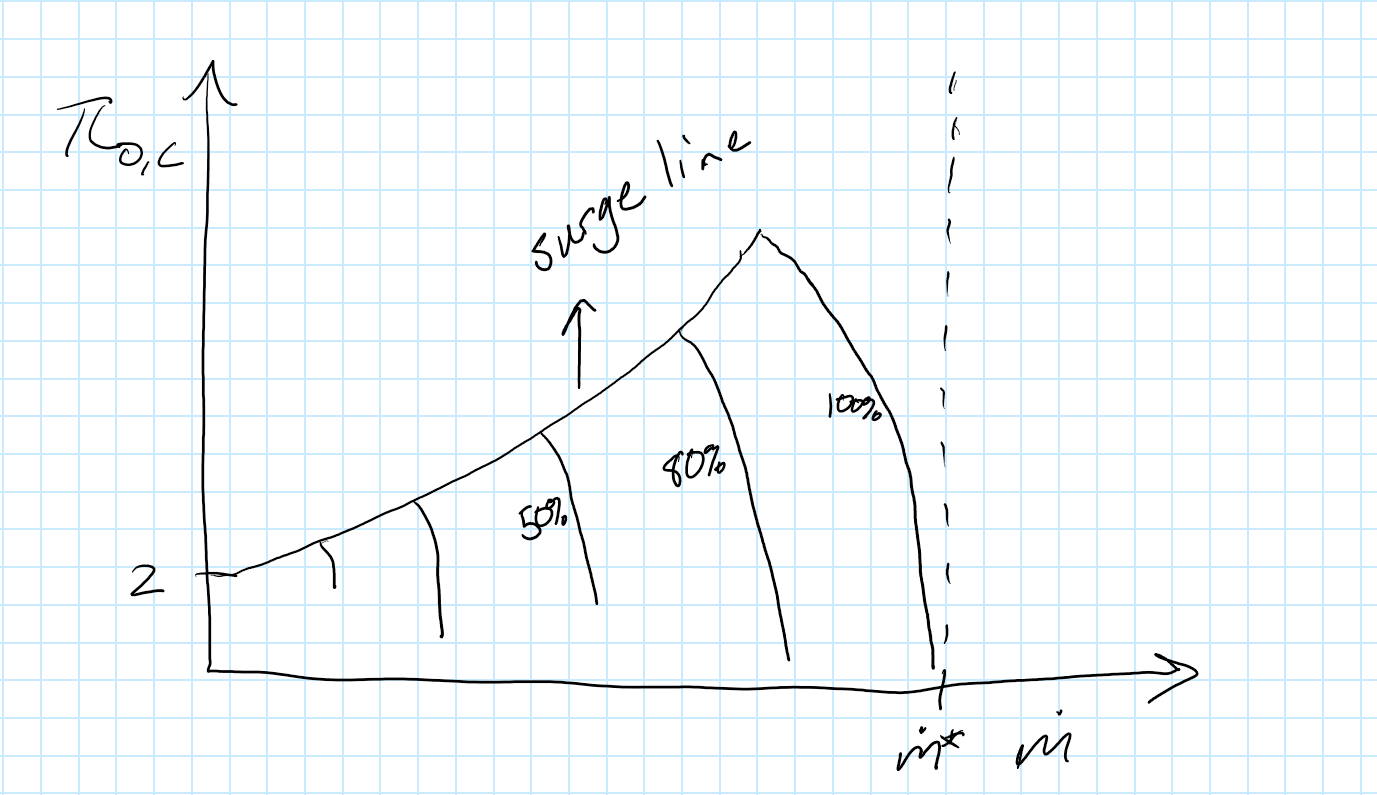
\includegraphics[width=\linewidth]{hand drawn compressor map.png}
The \(\dot{m}^*\) that I show on the graph is the point at which the compressor becomes sonically choked, and therefore limiting the 
maximum amount of mass flow rate.
\\ 
From Dimensionaless mass flow:
\[
\frac{\dot{m}\sqrt{R T_0}}{P_0 \sigma} = \sqrt{\gamma} M \left(1 + \frac{\gamma-1 }{2} M^2\right)^{\frac{-(\gamma+1)}{2(\gamma-1)}}
\]
Producing the choked mass flow rate of:
\[
\dot{m}^* = \frac{P_0 \sigma \sqrt{\gamma}}{\sqrt{R T_0}} \left(1 + \frac{\gamma-1 }{2}\right)^{\frac{-(\gamma+1)}{2(\gamma-1)}}
\]
\end{solutionorbox}


\end{questions}
\end{document}
